\section{Discussion}
\subsection{Discussion}
\begin{frame}{Limitations and insights}
    \begin{itemize}
        \item Low availability of data for some classes impact performance on certain findings.
        \item High sensitivity of our model to less frequent findings. (e.g. Local Asymmetries)
        \item Our model is able to identify findings regardless of scale of windows.
    \end{itemize}
\end{frame}


\subsection{Future Work}
\begin{frame}{Future Work}
    \begin{itemize}
        \item Study of unknown-to-model images for measurement of performance with local population.
        
        \begin{figure}
            \centering
            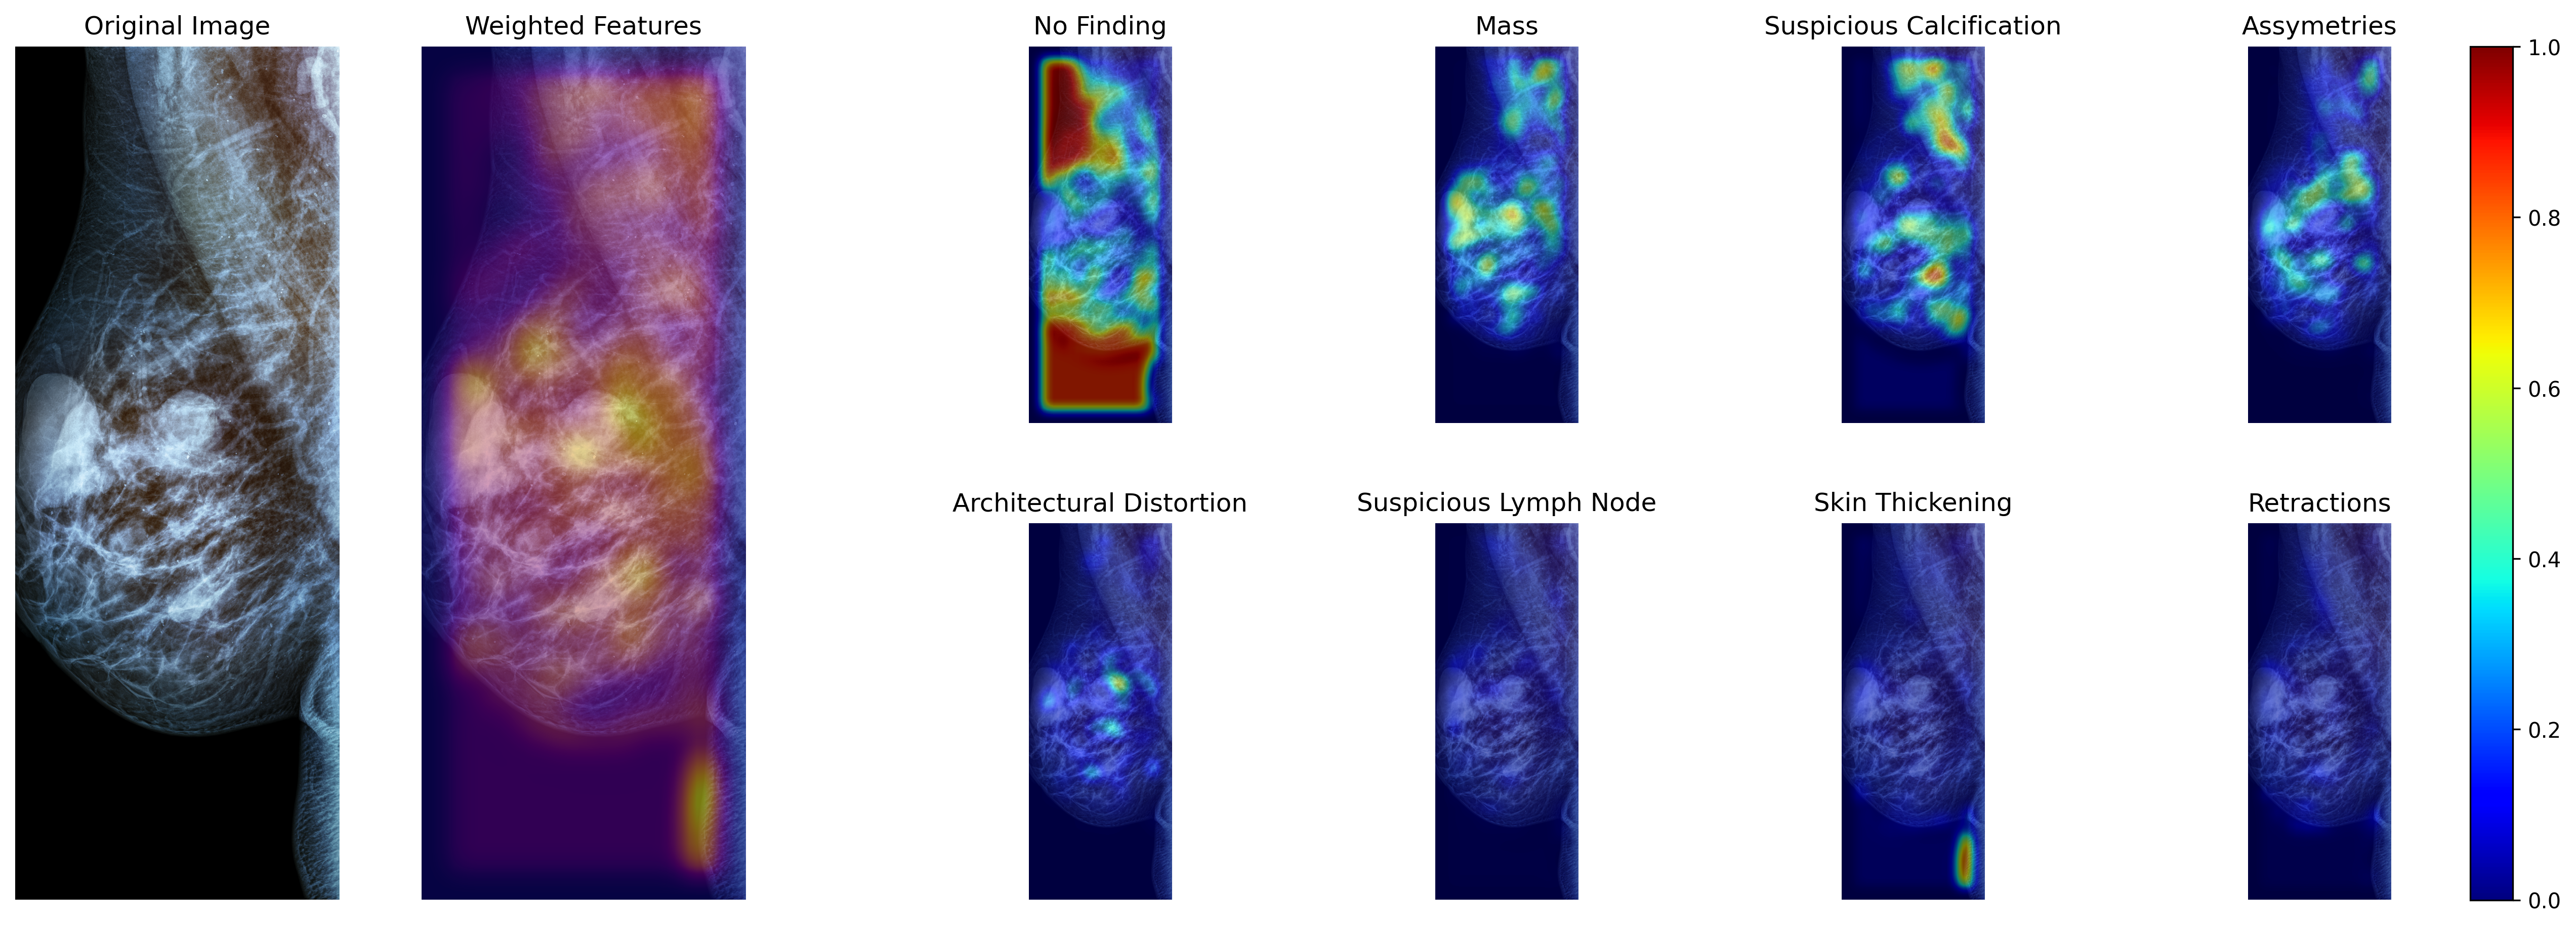
\includegraphics[height=0.45\textheight]{imagenes/predcmim_RMLO_7UTnE7GZPY.png}
            \caption{Right MLO image of Chilean patient}
        \end{figure}

        \item Analysis of selected features and their relationship with findings, in order to identify possible biases and discard of low-performance predictions.
    \end{itemize}
\end{frame}
